%!TEX root = main.tex
\section{Performance}
\label{sec:performance}
    At this point we started some simulations to check various performances. We mentioned in section \ref{sec:model_eval} that the models Logistic Regression, Random Forest and MLP were left over. Before we started the simulations we performed a few tests. The three models calculated probabilities for a specific market situation. Also a set of training data was given. MLP calculated probabilities which seemed not to be realistic. However, Logistic Regression and Random Forest showed good results. Therefore, we decided to not focus on MLP any more and compare the performance of Logistic Regression and Random Forest in the simulations.

\subsection{Pricewars Platform}
\label{sec:platform}
    In the winter term 2016/17 a master's project from the HPI has built a simulation platform. The main goal of this platform is to evaluate how different pricing strategies perform. Essentially, the platform is a marketplace environment where customers exist. The customers have behaviours that can be configured. Several merchants are already implemented as well. Thus, it is easy to let our own merchant compete against others. The application is based on a microservice architecture. Each merchant has an authentication token and REST requests are used to communicate.

\subsection{Simulations}
    We start the existing merchants Two Bound, Cheapest and Fix Price for the following simulations. The consumer performs 100 purchases per minute and is set to 100\% logit behaviour. The logit coefficients are shown in figure \ref{fig1}.
    \begin{figure}[ht]
    \centering
        \begin{tabular}{ l | c | r | r | r}
            interc. & price rank & \#competitors & avg price & quality rank \\
            \hline  
            -6.62 & 0.2 & 0.25 & -0.008 & -0.18 \\
        \end{tabular}
    \caption{Logit coefficients}
    \label{fig1}
    \end{figure}

    The universal model (section \ref{sec:universal_model}) is not used during the simulations. Because of that the charts can illustrate the learning effect of our approach better. Instead of the universal model the merchant sets random prices for the first learning interval. Thereby it generates an accurate training data set for the following price predictions. One learning interval takes two minutes. Figure \ref{fig2} shows that Random Forest chooses prices between 0.8 times and 3 times the purchase price (see section \ref{sec:random_prices}). The prices from the Cheapest and the Two Bound merchants are also influenced by the random prices. This interval is called exploration phase.
    
    \begin{figure}[ht]
        \centering
        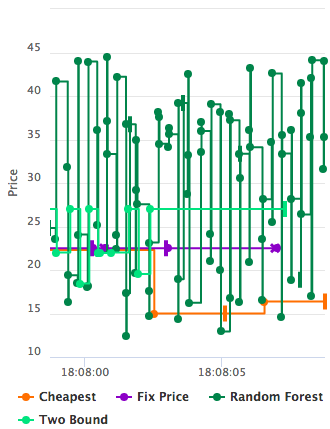
\includegraphics[width=0.35\textwidth]{img/rndmfrst_explor2.png}
        \caption{price chart exploration phase}
        \label{fig2}
    \end{figure}
 

\subsubsection{Logistic Regression Simulation}
    ~\\
    The Logistic Regression simulation begins with the exploration phase. This phase is similar to the Random Forest exploration phase from figure \ref{fig2}. Afterwards, the model has collected enough training data and the new best prices are predicted by the Logistic Regression model. You can see in figure \ref{fig3} that our merchants predicts the highest possible price as best price.

    \begin{figure}[ht]
        \centering
        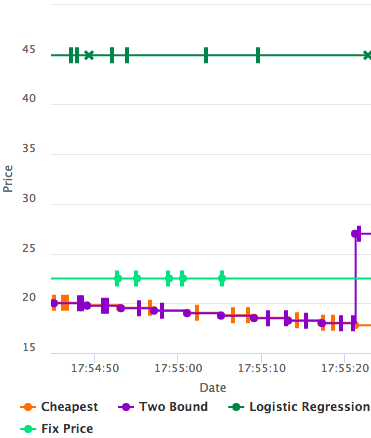
\includegraphics[width=0.35\textwidth]{img/logit_prices.png}
        \caption{price chart Logistic Regression}
        \label{fig3}
    \end{figure}

    The profit per minute is illustrated in figure \ref{fig4}. Logistic Regression has already during the exploration phase more profit per minute than the other merchants. When this phase ends (at the time 17:48:00) the profit per minute continues to grow.

    \begin{figure}[ht]
        \centering
        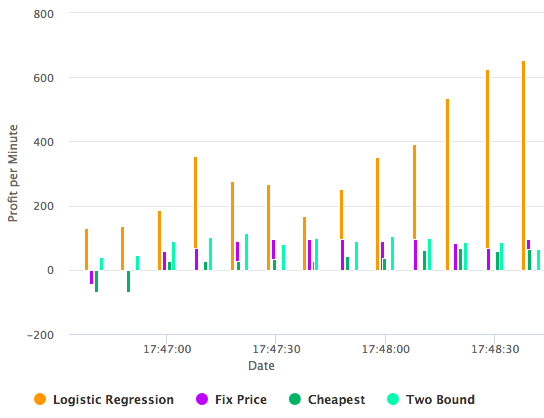
\includegraphics[width=0.45\textwidth]{img/logit_profit_per_min.png}
        \caption{profit per minute Logistic Regression}
        \label{fig4}
    \end{figure}

    At the end the Logistic Regression model is very successful with the strategy of just setting the highest possible price. Also the long term performance is quite good. Logistic Regression has approximately five to six times of revenue compared to the merchant with the second most.


\subsubsection{Random Forest Simulation}
    ~\\
    Figure \ref{fig5} shows the price chart of Random Forest after the exploration phase. In comparison to Logistic Regression the prices are not set to a constant price. The prices are still higher than the other merchants and for a short time the highest possible. These prices are regularly adjusted though.
    \begin{figure}[ht]
        \centering
        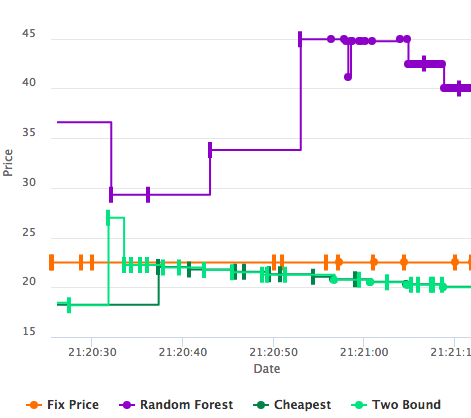
\includegraphics[width=0.45\textwidth]{img/rndmfrst_prices.png}
        \caption{price chart Random Forest}
        \label{fig5}
    \end{figure}

    Random Forest generates the most total profit. In figure \ref{fig6} this advantage is represented. But it is not as big as the advantage of Logistic Regression.

    \begin{figure}[ht]
        \centering
        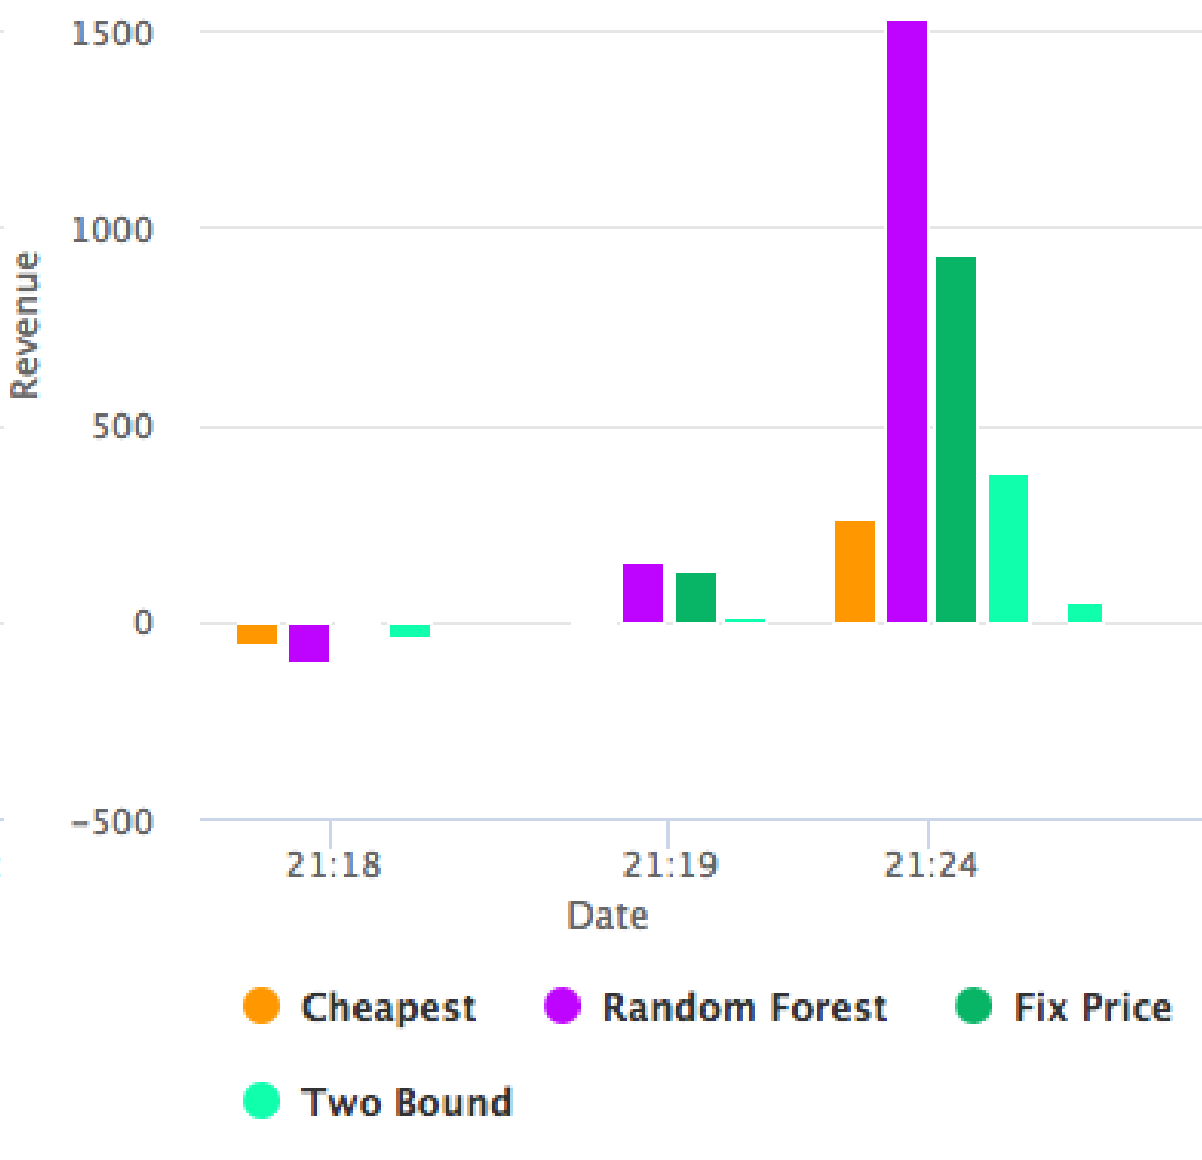
\includegraphics[width=0.4\textwidth]{img/rndmfrst_total_profit.png}
        \caption{total profit Random Forest}
        \label{fig6}
    \end{figure} 


\subsubsection{Logistic Regression vs. Random Forest}
    ~\\
    To see if our two different models influence each other we let them compete in the same simulation. After the exploration phase both models are deciding for the highest possible price (see figure \ref{fig7}).
    \begin{figure}[ht]
        \centering
        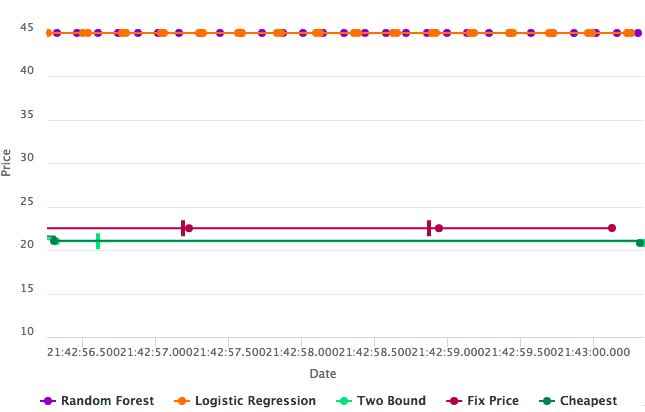
\includegraphics[width=0.5\textwidth]{img/prices_both.png}
        \caption{price chart both models}
        \label{fig7}
    \end{figure} 

    Thereafter Logistic Regression remains at this mark while Random Forest predicts other prices. Because of that Random Forest gains many sales with a low price and does not generate much profit. Figure \ref{fig8} shows the total profit.

    \begin{figure}[ht]
        \centering
        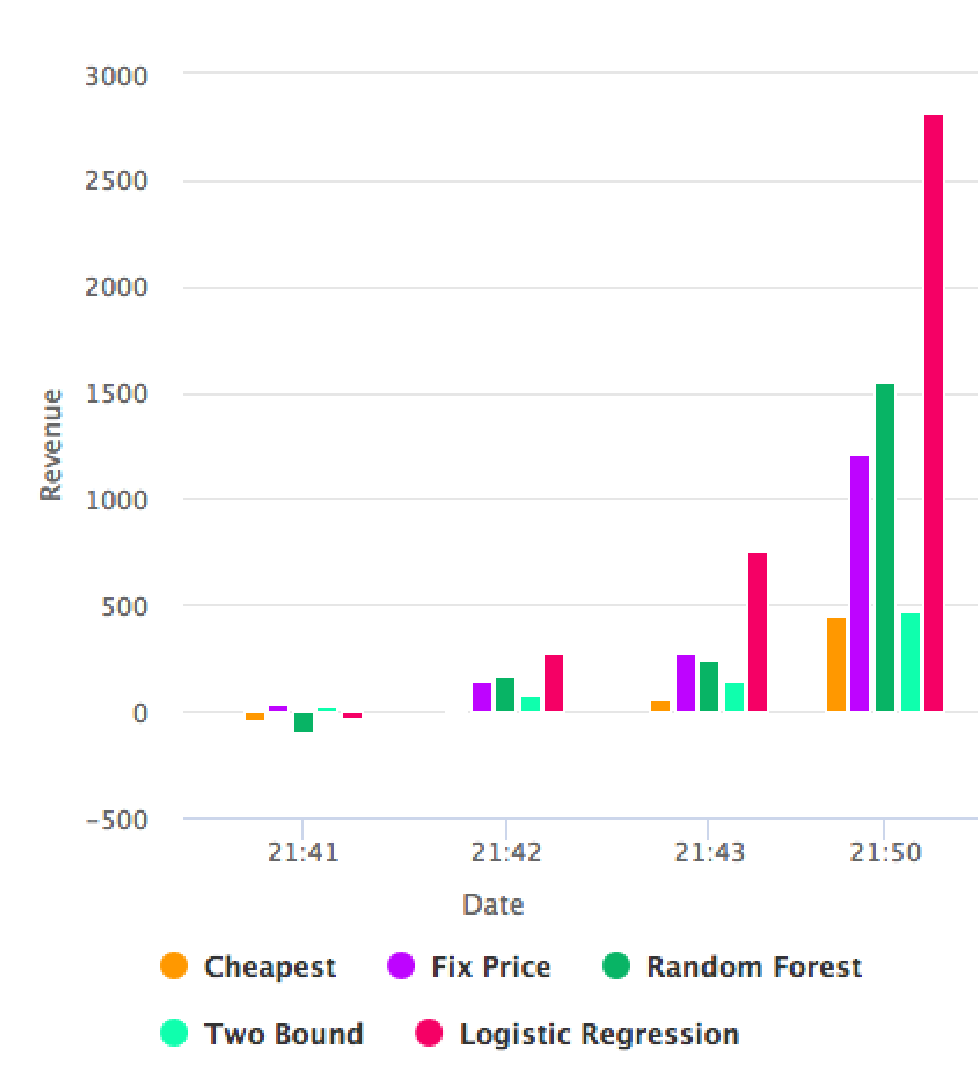
\includegraphics[width=0.45\textwidth]{img/total_profit_both.png}
        \caption{total profit both models}
        \label{fig8}
    \end{figure} 


\subsection{Drawback Logistic Regression}
    In the most cases our Logistic Regression performs great. The bad thing is that the models need good data to learn. If the Logistic Regression model remains at one price it is likely to get unbalanced training data at a point. For example, we made a simulation with a customer who only buys products from merchants with the lowest three prices. In the beginning Logistic Regression was placed at rank four. And there it remained because there was not enough training data for other prices. That is why we think that Random Forest fits better in most situations. Nonetheless, this problem could be solved by some additional rules for our Logistic Regression merchant (see section \ref{sec:future_work}).
